%%
%% This is file `example.tex',
%% generated with the docstrip utility.
%%
%% The original source files were:
%%
%% coppe.dtx  (with options: `example')
%% 
%% This is a sample monograph which illustrates the use of `coppe' document
%% class and `coppe-unsrt' BibTeX style.
%% 
%% \CheckSum{1391}
%% \CharacterTable
%%  {Upper-case    \A\B\C\D\E\F\G\H\I\J\K\L\M\N\O\P\Q\R\S\T\U\V\W\X\Y\Z
%%   Lower-case    \a\b\c\d\e\f\g\h\i\j\k\l\m\n\o\p\q\r\s\t\u\v\w\x\y\z
%%   Digits        \0\1\2\3\4\5\6\7\8\9
%%   Exclamation   \!     Double quote  \"     Hash (number) \#
%%   Dollar        \$     Percent       \%     Ampersand     \&
%%   Acute accent  \'     Left paren    \(     Right paren   \)
%%   Asterisk      \*     Plus          \+     Comma         \,
%%   Minus         \-     Point         \.     Solidus       \/
%%   Colon         \:     Semicolon     \;     Less than     \<
%%   Equals        \=     Greater than  \>     Question mark \?
%%   Commercial at \@     Left bracket  \[     Backslash     \\
%%   Right bracket \]     Circumflex    \^     Underscore    \_
%%   Grave accent  \`     Left brace    \{     Vertical bar  \|
%%   Right brace   \}     Tilde         \~}
%%
\documentclass[msc,
pdftex,
%doublespacing,
numbers]{coppe}
\usepackage[T1]{fontenc}
\usepackage{amsmath,amssymb}
\usepackage{lmodern}
\usepackage[utf8]{inputenc}
\usepackage[pt,showend]{programma}

\makelosymbols
\makeloabbreviations

\begin{document}
  \title{Utilização de uma metaheurística hibrida para solução do problema de construção de trilhos de aeronaves }
  \foreigntitle{Using a hybrid metaheuristic for solving the aircraft rotation problem}
 \author{Alexander}{de Almeida Pinto}
  \advisor{Prof.}{Nome do Primeiro Orientador}{Sobrenome}{D.Sc.}
  \advisor{Prof.}{Nome do Segundo Orientador}{Sobrenome}{Ph.D.}
  \advisor{Prof.}{Nome do Terceiro Orientador}{Sobrenome}{D.Sc.}

  \examiner{Prof.}{Nome do Primeiro Examinador Sobrenome}{D.Sc.}
  \examiner{Prof.}{Nome do Segundo Examinador Sobrenome}{Ph.D.}
  \examiner{Prof.}{Nome do Terceiro Examinador Sobrenome}{D.Sc.}
  \examiner{Prof.}{Nome do Quarto Examinador Sobrenome}{Ph.D.}
  \examiner{Prof.}{Nome do Quinto Examinador Sobrenome}{Ph.D.}
  \department{SDI}
  \date{1}{2011}

  \keyword{Transporte}
  \keyword{PCTA}
  \keyword{Metaheurística}
  \keyword{Método Exato}
  \keyword{GRASP}
  \keyword{Rotas de Aeronaves}
  
  \maketitle

  \frontmatter
  
  \dedication{A minha família e amigos cuja valia é imensurável.}

  \chapter*{Agradecimentos}

  Gostaria de agradecer a todos que fizeram 

  \begin{abstract}

  Apresenta-se, nesta tese, ...

  \end{abstract}

  \begin{foreignabstract}

  In this work, we present ...

  \end{foreignabstract}

\tableofcontents
\listoffigures
%\listoftables
\printloabbreviations
\printlosymbols

\mainmatter
  
\chapter{Introdução}
  
 A aviação é o principal meio de transporte de pessoas e de mercadorias capaz
 de atravessar grandes distâncias além de ser fundamental para o crescimento
 da economia e do turismo mundial contribuindo assim para a melhora da
 qualidade de vida das pessoas proporcionando lazer e experiências com outras
 culturas. O uso da aviação comercial tem crescido significativamente nas
 últimas décadas e a previsão é que esse aumento seja cada vez maior, pelo
 menos no Brasil, que está fazendo um grande investimento para ampliar e
 melhorar a infraestrutura aeroportuária com a finalidade de atender a grande
 demanda que é esperada para a Copa do Mundo de 2014 e para as Olimpíadas de
 2016. Além disso a economia do país está crescendo e provocando um aumento da
 renda e da qualidade de vida incentivando as pessoas a viajar e explorar novas
 oportunidades.

%Pode se falar também do aumento da confiança no setor aereo que está sendo
% associado a uma forma segura de viajar.
  	
Esse ambiente favorável tem provocado o aumento do número de companhias
aéreas, fazendo com que ocorra uma maior competição e assim a necessidade de
otimizar a utilização dos recursos disponíveis, reduzindo os custos para
poder continuar a crescer e oferecer tarifas mais competitivas. Porém os
problemas presentes na indústria aeronáutica são complexos envolvendo
múltiplas decisões conflitantes que precisam ser otimizadas em conjunto.
Diversas técnicas são desenvolvidas e utilizadas para tentar melhorar o
planejamento e a operação das empresas aéreas. Muitas dessas técnicas estão
disponíveis na literatura científica, nos campos da pesquisa operacional e da
matemática e normalmente são modelados para funcionar em sistemas
computadorizados de alta capacidade com a finalidade de automatizar, ou pelo
menos auxiliar a tomada de decisões. Essas técnicas se tornam mais
necessárias a medida que a empresa aérea cresce e a tomada de decisão,
baseada nos julgamentos individuais e nas experiências, se tornam mais
difíceis \cite{ahmed2009}.
  	
  	
Os principais problemas relacionados dizem respeito ao planejamento, envolvendo
a criação de linhas de trabalho tanto para as aeronaves quanto para a
tripulação. O objetivo costuma ser a minimização dos custos operacionais ou a
maximização dos rendimentos. Custos operacionais consiste, por exemplo, nos
custos envolvidos com combustíveis, óleo, taxas de aterrissagem. Também pode
ser levado em consideração a perda de rendimentos com a utilização de aeronaves
com menos assentos do que a demanda de passageiros. Fatores como o bem
estar dos passageiros também pode ser levado em consideração, provocando por
exemplo a uma redução na quantidade de conexões e de escalas.
	
Para que seja possível ter uma visão geral do contexto é necessário descrever os
problemas que estão associados com a construção de trilhos de aeronaves. O
primeiro dos problemas que será tratado aqui é a modelagem de mercado que tem
como objetivo de fazer o levantamento da quantidade de passageiros que tem
interesse em viajar entre as localidades e em qual espaço de tempo,
adicionalmente pode-se criar demandas através da criação de novas rotas com o
auxilio de propagandas. Essa demanda normalmente apresenta uma grande variedade
dependendo da época do ano e o levantamento desses dados de forma errada pode
causar grandes prejuízos. É importante categorizar o tipo de passageiro para
poder fazer escolhas futuras que não levem em consideração apenas fatores
quantitativos.

Posterior a modelagem de mercado tem-se a necessidade de definir qual
equipamento (frota) irá operar cada trecho definido pela
demanda \cite{pimentel2005}, esse problema é conhecido como a atribuição de
frota (\textit{Fleet Assigment Problem}) . A definição de um equipamento errado
pode provocar a subutilização da aeronave o que provocaria prejuízos ou a
superutilização que provocaria insatisfação dos clientes. Ao final dessa etapa
irão ser formados conjuntos de voos que deverão ser operados por tipos de
aeronaves específicas. É a partir desses conjuntos que deverá ser feito a
construção dos trilhos das aeronaves.

Um trilho de aeronave é a sequência de voos que uma aeronave deve operar em um
determinado período, e o problema de construção desses trilhos 
(\textit{Aircraft Rotation Problem}) tem como objetivo principal a redução do
número de aeronaves necessários para operar todos os voos e como objetivo
secundário fazer o menor número de modificações possíveis no planejamento inicial desses
voos.

O passo seguinte utiliza das sequencias de voos do passo anterior para construir
o melhor conjunto de pairings\footnote{Pairing é o conjunto de voos
que pode ser operados por uma tripulação sem que seja violada qualquer
regra da legislação vigente e que ao final do último voo o tripulante
esteja de volta a sua cidade base.} de forma que cada voo seja coberto por
pelo menos um pairing. Gastos com alojamentos, alimentação, transporte em terra
e deadheads\footnote{Deadhead é o voo que o tripulante viaja sem trabalhar,
com a finalidade de transporte para outra localidade normalmente para sua
base ou para suprir uma nova demanda, o deadhead pode ser operado por
aviões de outras companhias, nesse caso o custo dessa viagem é maior.} devem
ser levados em consideração. A partir desse conjunto é feito a escala dos
tripulantes (\textit{Crew Scheduling Problem}) que atribui os pairings a
tripulação acrescentando as atividades de solo, tais como \textit{Call
Time}\footnote{Call time é o tempo que a tripulação tem para se apresentar a
companhia aérea antes de iniciar de fato seu turno de trabalho.},
\textit{Stand-by duties}\footnote{Stand-by duties
são turnos em que o tripulante fica a disposição da companhia aérea afim de
suprir possíveis eventualidades.} e os dias de descanso. O objetivo dessa ultima
etapa é fazer uma distribuição da forma mais justa possível, tentando balancear
a quantidade de trabalho (horas a serem voadas) entre os tripulantes e também
tentar cumprir as preferencias dos tripulantes sem violar nenhuma restrição da
legislação trabalhista em vigor.
   

Esse trabalho mostra uma forma eficiente de resolver o Problema de Construção
de Trilhos de Aeronaves (PCTA) 
%\abbrev{PCTA}{Problema de Construção de Trilhos de Aeronaves} 
que também é conhecido na literatura como Aircraft Rotation
Problem (ARP) 
%\abbrev{ARP}{Aircraft Rotation Problem}
. O PCTA é um dos
principais problemas presentes na industria da aviação e seu objetivo
é fazer o sequenciamento dos voos de cada frota da companhia de forma que seja
possível opera-las com o menor número de aeronaves possíveis\citep{abiliolivro}
bem como efetuar a menor modificação possível no planejamento inicial dos voos.
Cada sequência de voos recebe o nome de trilho de aeronave e o conjunto desses
trilhos é denominado de malha aérea. 

Para resolver o PCTA foram aplicados técnicas de metaheurísticas combinadas com
o método exato de programação linear através da criação de um modelo matemático
simplificado.

Essa estratégia foi escolhida pois com os computadores atuais não é possível
obter resultados com a aplicação apenas do modelo, que retorna o resultado
ótimo, pois o tempo necessário para resolver instâncias semanais do PCTA já é
considerado inviável. A utilização apenas de metaheurística foi uma alternativa
que foi levada em consideração no início, porém nos resultados práticos a
qualidade da solução se mostrou muito aquém da desejada. Dessa forma surgiu a
idéia de mesclar as duas técnicas, com a finalidade de obter a convergência do
modelo e a velocidade da metaheurística.

Na literatura tem-se observado um crescimento no número de trabalhos que se
utilizam de metaheurísticas híbridas como método de resolução de problemas
complexos de otimização combinatória apresentando soluções de alta qualidade
(ACRESCENTAR CITAções). Esse fato também aconteceu na resolução do PCTA.



%Para resolver o PCTA, devemos estar cientes de algumas restrições que envolvem
%tempo e espaço. Por exemplo, um voo não pode iniciar antes da chegada do voo
%que lhe antecede, nem de um local diferente da cidade de destino deste voo
%antecessor, esses exemplos são denominados respectivamente de restrições
%temporais e geográficas do problema. Há também a restrição de que um voo deve
%permanecer em solo, entre conexões, por um período de tempo que seja suficiente
%para fazer a troca de passageiros e abastecimento da aeronave e quando for o
%caso para a mudança da tripulação, esse tempo varia de acordo com o aeroporto e
%com o tipo de aeronave.

%Existe também a restrição de consistência que está presente em instâncias que
%possuem frequência. Nessas instâncias um voo pode aparecer em diversos dias.
%Dessa forma deve-se garantir que o horário de partida desse voo seja o mesmo em
%todos os dias que ele ocorrer, ou seja, caso alguma modificação seja feita no
%horário de partida sugerido desse voo, em um dos dias, então todos os outros
%dias da frequência também devem ser modificados.

%Outro aspecto importante diz respeito às restrições de manutenção. Sabe-se que
%um avião deve ter checagens periódicas. Oportunidades de realizar essas tarefas
%ocorrem apenas em algumas conexões potencialmente disponíveis. Como
%consequência, uma sequência de voos deve ser construída de forma que essas
%restrições não sejam violadas. A fim de incorporar essas restrições facilmente
%ao nosso framework, assumimos que as rotações são designadas a tipos não
%específicos de aeronave. Dessa forma, se uma aeronave tem necessidade de
%manutenção, um voo especial é criado com origem e destino na base de manutenção
%escolhida e com a sua duração exatamente igual ao tempo de manutenção 
%\cite{pontes2002}.

%	Vale ressaltar ainda que na resolução do PCTA deve-se levar em consideração as
%	particularidades especificas de cada companhia aérea como o número de aviões
%disponíveis na frota, o atraso máximo permitido nos voos, a quantidade máxima
%de voos que podem sofrer atraso, o número máximo de voos que podem ser
%cancelados, o número máximo de voos de reposicionamento que podem ser criados
%entre outros.
	
%De uma maneira geral, o principal objetivo do PCTA é a minimização do número de
%trilhos seguido da minimização do custo total dos trilhos gerados. Esse custo
%pode envolver diversos componentes, sendo o tempo médio diário de utilização
%das aeronaves um dos mais importantes \citep{abiliolivro}.
 
%###################################### 
%Aqui já nao descreve mais o problema.
%######################################
  
Nos dias de hoje, com o avanço da tecnologia e o aumento da competitividade
desenvolver soluções com melhor qualidade acaba se tornando um fator decisivo
para a permanência no mercado, tornando-se então necessário a obtenção de
soluções de forma mais rápida, mais barata e utilizando menos recursos. Por
causa da dificuldade que é inerente a essa classe de problemas a qualidade das
soluções obtidas manualmente são muito inferior em relação a melhor solução
possível. Outra característica que reforça a necessidade da obtenção de melhores soluções é o
aumento do tamanho e da complexidade das instâncias trabalhadas. A partir desse
cenário pode-se perceber a necessidade de utilização de técnicas de otimização.

  
%As metaheurísticas podem ser definidas como um conjunto de procedimentos de
%caráter geral, com capacidade de guiar o procedimento de busca, tornando-o
%capaz de escapar de ótimos locais. Elas têm como objetivo, encontrar uma
%solução tão próxima quanto possível da solução ótima do problema com baixo
%esforço computacional. Em geral, as metaheurísticas são bastante utilizadas na
%resolução de problemas de otimização. Esses problemas, também conhecidos como
%problemas NP-difíceis\abbrev{NP}{Non-Polinomial}, podem ser definidos como um
%conjunto de problemas para os quais ainda não existe um algoritmo que os
%resolvam de forma exata e em tempo polinomial \citep{maritan2009}. Para esses
%tipos de problemas o uso de métodos exatos é bastante restrito, uma vez que o
%esforço computacional para encontrar uma solução exata em instâncias reais é
%consideravelmente alto. Na prática, no entanto, é suficiente encontrar uma
%solução melhor que a utilizada no ambiente operacional.


%#############################################
%{\large >>>> Descrever em que tem se baseado a solução desse problema na literatura <<<<}
%Essa parte deveria ir para a revisão da literatura.
%#############################################

Em relação ao PCTA a literatura pesquisada \cite{ahmed2009} \cite{arguelo1007}
\cite{cordeau2001} \cite{mohamed2011} \cite{abiliolivro} mostra uma grande quantidade de
tentativas de resolver o problema utilizando modelagens matemáticas, que apesar
de garantir a solução ótima não se mostra viável para resolver grandes
instâncias. Alguns trabalhos mostram a similaridade desse problema com o
problema do caixeiro viajante assimétrico \cite{clarke97}. E outros resolvem
uma parte do problema utilizando metaheurísticas \cite{arguelo1007}. Além disso,
a pesquisa constatou que a literatura acerca do PCTA não disponibiliza as
instâncias que foram trabalhadas dificultando assim a comparação dos
resultados obtidos com esses trabalhos, logo um dos objetivos desse trabalho é
disponibilizar um conjunto de instâncias.

%#############################################
%{\large	>>>> Fazer uma breve descrição de programação linear, maiores detalhes serão dados na fundamentação teórica. <<<<	}
%#############################################

Atualmente existem diversas fontes na qual se podem obter instâncias para
problemas de otimização combinatória sendo uma das mais conhecidas a
OR-Library \footnote{ A OR-Library pode ser acessado em
http://people.brunel.ac.uk/~mastjjb/jeb/info.html} que foi descrito
inicialmente em J.E.Beasley \cite{orlibrary} permitindo o acesso a centenas de
conjuntos de instâncias a partir da Internet.
  
Apesar da existência dessas entidades apenas uma instância, a da Rio Sul, foi
encontrada em um relatório técnico da UFPB. Com a finalidade de ter outra
instância, foi feito em dezembro de 2010 o levantamento dos voos operados pela
compahia denominada TAM (http://www.tam.com.br). Esse levantamento foi feito
atarvés de uma pesquisa observativa através do comparativo da malha operada
pela companhia, que pode ser visto na Figura \ref{fig:malhatam}, e as
possibilidades de voos diretos do equipamento AirBus Industrie A310, que era a aeronáve com a maior frota da
empresa.
	
\begin{figure}[ht]
\caption{Rotas de voo da companhia aérea TAM. \mbox{Fonte:
(http://www.airlineroutemaps.com/)}}
\label{fig:malhatam}
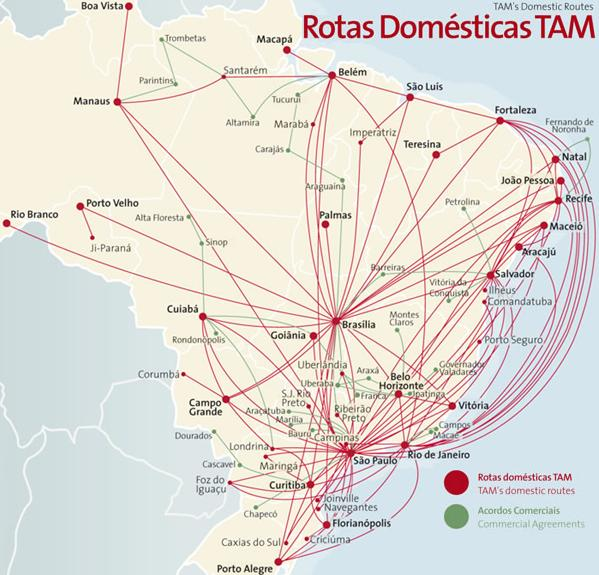
\includegraphics[scale=0.45]{./img/tam_brazilian_airlines}
\end{figure}
	
A malha da Rio Sul se refere a uma instância com voos de um dia de operação da
empresa contendo 107 voos, onde na prática era operado com 20 trilhos
que eram formados manualmente \cite{pontes2002}. A malha da TAM, que foi obtida
manualmente, é formada por 241 voos que possuem uma grande quantidade de
ligações entre os 31 aeroportos envolvidos, dessa forma o grau de complexidade
dessa instância se mostrou mais complexa. 

Essas instâncias foram estendidas para o período de uma semana para testar o
comportamento do algoritmo e do solver. Dessa forma a instância da Rio Sul
estendida apresentou 749 voo e a da Tam estendida ficou 1687 voos.
	
O maior interesse desse trabalho se encontra em instâncias locais
pois as instâncias de outras grandes empresas globais apresentam a
característica hub-and-spoke, que pode ser vista na Figura
\ref{fig:hubandspoke}. Uma malha é caracterizada como sendo do
tipo hub-and-spoke se ela apresentar uma grande concentração de voos em poucos
aeroportos e adicionalmente se um voo tem ligação com um hub ele não poderá ter
ligação com outros hubs a não ser que ele também seja um hub.
Instâncias com essa caractéristicas são mais fáceis de serem
resolvidas pois não apresentam a caractéristica explosiva no nível das malhas
de voos heterogêneas presente nas malhas de voos brasileiras.
	
\begin{figure}[ht]
\caption{Malha hub-and-spoke. \mbox{Fonte: (Própria)}}
\label{fig:hubandspoke}
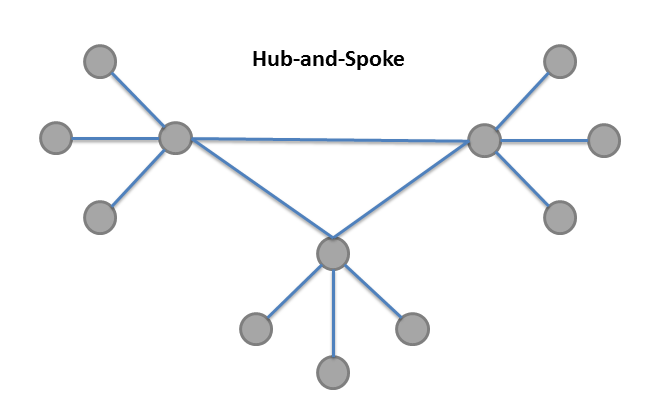
\includegraphics[scale=0.35]{./img/hubandspoke}
\end{figure}
 	 	
	
Novas instâncias reais não foram possíveis devido a falta de contato entre as
empresas e a acadêmia. Grande parte dessa falta de comunicação se deve ao receio
de revelar dados que podem vir a lhes prejudicar junto a concorrência.

Essas instâncias podem ser vistas nos anexos ao final desse trabalho.


\section {Objetivos do trabalho}

% Falar das consequências dos objetivos (em termo de economia e em relação a
% melhora do trafego aereo, no brasil, pois irá fazer com que as aeronáves
% fiquem mais tempo voando. O principal problema hoje é na falta de espaço no
% solo para pousar os avioes.

\subsection{Primário}
Tendo em vista os aspectos apresentados, o objetivo principal dessa proposta de
trabalho consiste no desenvolvimento de um método híbrido baseado nas
metaheurísticas GRASP e ILS e em programação linear inteira para a resolução do
problema construção de trilhos de aeronaves (PCTA) cobrindo todos os voos
planejados com o menor número de aeronaves bem como efetuando a menor mudança
possível no planejamento inicial desses voos. O método proposto tem a finalidade
de explorar a eficiência computacional, e irá ser combinada com etapas de
refinamentos composta por métodos exatos para acelerar a convergência e
adicionalmente fugir de mínimos locais.

\subsection{Secundário}

Esse trabalho também visa a disponibilização de um conjunto de instâncias que
irá permitir uma melhor comparação que poderá ser efetuada por trabalhos
futuros.

Adicionalmente disponibilizaremos uma interface que irá permitir ao usuário a
utilização de forma fácil do algoritmo com uma visualização do resultado através
de um gráfico de gantt.

\section {Organização da proposta }

O trabalho está estruturado da seguinte forma:

\begin{itemize}

\item Capítulo 1: Apresenta a motivação e as vantagens de resolver o PCTA
utilizando uma técnica híbrida com metaheurísticas e programação linear e
enfatiza a importância desse problema na indústria aeronáutica. Ao final os
objetivos do trabalho são descritos.

\item Capítulo 2: Apresenta a fundamentação sobre a otimização, metaheurísticas
e programação linear. Na seção referente à otimização além da descrição serão
discutidos heurísticas construtivas. A seção referente às metaheurísticas irá
iniciar com uma descrição seguida do detalhamento das metaheurísticas
utilizadas no trabalho, como o GRASP e o ILS. Ao final da fundamentação teórica
será feita uma revisão dos principais trabalhos relacionados ao presente
trabalho que estão presentes na literatura.

\item Capítulo 3: Mostra como foi obtida a malha da companhia de transporte aéreo TAM e qual a estratégia será utilizada para geração das novas instâncias.

\item Capítulo 4: Descreve o problema, explicando os conceitos que serão utilizados no trabalho.

\item Capítulo 5: Introduz o modelo matemático que foi desenvolvido.

\item Capítulo 6: Descreve o método proposto nesse trabalho, mostrando como foi feita a integração das metaheurísticas e da programação linear inteira e também descreve os parâmetros e as restrições que foram utilizadas.

\item Capítulo 7: Apresenta alguns resultados preliminares que já foram obtidos com o solver, dá diretrizes de como utilizar o método proposto e indica o que se espera ter para finalizar o trabalho.
%\item Capítulo 8: Dá uma conclusão, indicando o que tem que ser melhorado e o que se espera ter para a finalização do trabalho.

\item No final é apresentado a bibliográfia estudada, o cronograma de trabalho proposto durante os 24 meses de mestrado e os anexos que contém um maior detalhamento das instâncias e dos resultados obtidos.

\end{itemize}
\chapter{Fundamentação Teórica}

  Nesse capítulo será feita a fundamentação dos principais assuntos presentes nesse trabalho: a heurística construtiva, as metaheurísticas e a programação linear. Nas seções seguintes serão descritas os aspectos teóricos e os principais métodos relacionados a esse trabalho.

	\section{Heurísticas Construtivas}
		As técnicas de resolução heurísticas se utilizam de processos intuitivos com a finalidade de obter uma boa solução, a um custo computacional aceitável, ou seja não garante a otimalidade de um problema. O objetivo é obter em um tempo reduzido uma solução tão próxima quanto possível do ótimo global. 
		
		Uma heurística é dita construtiva quando a construção da solução se dá elemento por elemento. A forma de escolha dos elementos variam de acordo com a estratégia e a função de avaliação adotada, essa escolha deve levar em consideração o benefício da inserção de cada elemento para a solução final, escolhendo sempre o \emph{melhor} elemento em cada passo.
		
		O Algoritmo \ref{alg:heurconsgulosa} mostra o pseudocódigo para a construção de uma solução inicial para um problema de otimização que utiliza uma função gulosa \emph{g(.)}. Nesta figura, \emph{$t_{melhor}$} indica o membro do conjunto de elementos candidatos com o valor mais favorável da função de avaliação \emph{g}, isto é, aquele que possui o menor valor de \emph{g} no caso de o problema ser de minimização ou o maior valor de \emph{g} no caso de o problema ser de maximização.


\begin{pgrm}[h]
\begin{programma}
\ALGORITHM{$ConstruçãoGulosa(g(.), s$)}
\STATE s \GETS $\emptyset$;
\STATE Inicialize o conjunto $C$ de candidatos;
\WHILE{$C \neq \emptyset$}
\STATE $g(t_{melhor}) = melhor\{g(t) \mid t \in C\}$;
\STATE $s \GETS s \cup \{t_{melhor}\}$;
\STATE Atualize o conjunto $C$ de elementos candidatos;
\ENDWHILE
\STATE\RETURN $s$;
\ENDALGORITHM
\end{programma}
\caption{Heurística de construção gulosa de uma solução inicial}\label{alg:heurconsgulosa}

\end{pgrm}		
		

Uma outra forma de obter uma solução inicial é escolhendo os elementos candidatos aleatoriamente. Isto é, a cada passo, o elemento a ser inserido na solução é aleatoriamente selecionado dentre o conjunto de elementos candidatos ainda não selecionados. A grande vantagem desta metodologia reside na simplicidade de implementação. Segundo testes empíricos , a desvantagem é a baixa qualidade, em média, da solução final. Essa técnica é recomendada quando a característica do problema torna mais fácil o refinamento do que a construção de uma solução \citep{notasmarcone}. 

O Algoritmo \ref{alg:heurconsaleatoria} mostra o pseudocódigo para a construção de uma solução inicial aleatória para um problema de otimização.

\begin{pgrm}[h]
\begin{programma}
\ALGORITHM{$ConstruçãoAleatória(g(.), s$)}
\STATE s \GETS $\emptyset$;
\STATE Inicialize o conjunto $C$ de candidatos;
\WHILE{$C \neq \emptyset$}
\STATE Escolha aleatoriamente $t_{escolhido} \in C$;
\STATE $s \GETS s \cup \{t_{escolhido}\}$;
\STATE Atualize o conjunto $C$ de elementos candidatos;
\ENDWHILE
\STATE\RETURN $s$;
\ENDALGORITHM
\end{programma}
\caption{Heurística de construção aleatória de uma solução inicial}\label{alg:heurconsaleatoria}
\end{pgrm}

Para melhores resultados essa etapa deve ser seguida de um refinamento, pois a solução, quando gerada aleatoriamente, não costuma ser de boa qualidade.

\section{Metaheurística}

A utilização de métodos exatos para a resolução de problemas reais envolvendo otimização combinatória é restrito. Isso acontece pois com o aumento das instâncias envolvidas, o número de soluções possíveis cresce exponencialmente, fazendo com que as operações necessárias para a sua resolução não possa feita em tempo viável com os computadores atuais.  

Para contornar essa limitação e obter soluções para esses tipos de problemas, os pesquisadores desenvolveram técnicas que são capazes de guiar o procedimento de busca e assim encontrar boas soluções \cite{maritan2009}. Esses algoritmos, denominados heurísticas, encontram essas soluções utilizando pouco recursos computacionais, porém não garantem a solução ótima do problema \cite{dias2006}. Na prática, geralmente, uma boa solução é suficiente, já que a tomada de decisão tem que acontecer em um curto espaço de tempo.

As heurísticas só se aplicam a uma classe restrita de problemas. Para contornar essa restrição, foram desenvolvidas técnicas mais generalistas que foram denominadas de metaheurísticas. As metaheurísticas podem ser definidas como sendo um método heurístico para resolver de forma genérica problemas de otimização com a capacidade de escapar de ótimos locais. A idéia utilizada, normalmente, é obtida de algum evento natural como sistemas biológicos, da física, da inteligência artificial entre outros.

As metaheurísticas podem explorar o espaço de soluções basicamente de duas formas: as metaheurísticas de busca local e as metaheurísticas de busca populacional. Nas metaheurísticas de busca local, o procedimento de busca utiliza uma solução como ponto de partida em cada iteração. As metaheurísticas GRASP, Arrefecimento simulado (Simulated Annealing), Busca Tabu e ILS podem ser citadas como exemplos de metaheurísticas ponto-a-ponto. Nas metaheurísticas de busca populacionais, soluções de boa qualidade são combinadas com o intuito de produzir soluções melhores. Podemos citar como exemplo de métodos populacionais, os Algoritmos Genéticos, Colônia de Formigas (Ant Colony System), Núvem de Particulas (Particle Swarm Optimization) e etc \cite{maritan2009}.

Nesse trabalho foram utilizados as metaheurísticas de busca local GRASP e ILS de forma híbrida. As próximas seções descrevem essas metaheurísticas.

\subsection{GRASP}

Essa seção descreve a metaheurística GRASP (Greedy Randomized Adaptive Search Procedure - Procedimento de busca adaptativa gulosa e randômica), que foi proposto por Feo e Rezende \cite{resende1995}, e cujos conceitos serão utilizados na metodologia proposta para resolução do PCTA.
A metaheurística GRASP é um método iterativo do tipo \textit{multi-start} formado por duas fases: uma fase de construção de uma solução e outra de busca local. A fase de construção objetiva gerar uma solução viável para o problema proposto. E a fase de busca local na qual um ótimo local na vizinhança da solução construída é pesquisado. A melhor solução encontrada, ao longo de todas as iterações GRASP realizadas, é retornada.

O pseudo-código descrito no Algoritmo \ref{alg:grasp} ilustra um procedimento GRASP para um problema de minimização. Na linha 1 o custo da função objetivo da melhor solução encontrada é inicializada com $\infty$. A linha 2 repete o procedimento de construção e refinamento $GRASPMax$ vezes, por causa dessa etapa que o GRASP é considerado \textit{multi-start}.

Na linha 3 e 4 são feitas respectivamente a construção e a busca local que são representadas nos Algoritmos \ref{alg:graspcons} e \ref{alg:grasplocal} e serão detalhadas mais adiante.

Nas linhas 5 à 8, se a solução obtida na busca local for melhor que a melhor solução obtida até o momento ($f(s) < f{*}$) então são atualizadas respectivamente a solução e o custo relativo a função objetivo dessa solução. 
A linha 9 encerra as iterações do GRASP e a linha 10 retorna a melhor solução obtida.

\begin{pgrm}[h]
\begin{programma}
\ALGORITHM{GRASP($f(.), g(.), N(.), GRASPMax, s$)}
\STATE f{*} \GETS $\infty$;
\FOR{$1, 2, ..., GRASPMax$}
\STATE Construção($g(.), \alpha, s$);
\STATE BuscaLocal($f(.),N(.),s$);
\IF{$f(s) < f{*}$}
\STATE $s{*} \GETS s$;
\STATE $f{*} \GETS f(s)$;
\ENDIF
\ENDFOR
\STATE\RETURN $s{*}$;
\ENDALGORITHM
\end{programma}
\caption{Procedimento GRASP.}\label{alg:grasp}
\end{pgrm}

Na fase de construção uma solução é iterativamente construída, elemento por elemento. A parte gulosa da função visa gerar uma solução factível de melhor custo. O componente aleatório é incluído para explorar
regiões diversas do espaço de soluções e é uma das chaves da efetividade do GRASP.

A fase de construção do GRASP é baseada na construção de uma lista restrita de candidatos (LCR). Essa lista contem os melhores candidatos que podem ser adicionados a solução em um dado momento, a quantidade de elementos dessa lista é regulada pelo $\alpha$ que é um dos parâmetros do GRASP. O $\alpha$ é definido como sendo o nível de aleatoriedade da solução.

\begin{pgrm}[h]
\begin{programma}
\ALGORITHM{$Construção(g(.), \alpha,s$)}
\STATE s \GETS $\emptyset$;
\STATE Inicialize o conjunto $C$ de candidatos;
\WHILE{$C \neq \emptyset$}
\STATE $g(t_{min}) \GETS min\{g(t) \mid t \in C\}$;
\STATE $g(t_{max}) \GETS max\{g(t) \mid t \in C\}$;
\STATE $LCR \GETS \{t \in C \mid g(t) \leq g(t_{min}) + \alpha(g(t_{max}) - g(t_{min}))\}$;
\STATE Selecione aleatoriamente um elemento $t \in LCR$;
\STATE $s \GETS s \cup \{t\}$;
\STATE Atualize conjunto de candidatos;
\ENDWHILE
\STATE\RETURN $s$;
\ENDALGORITHM
\end{programma}
\caption{Procedimento de construção do GRASP.}\label{alg:graspcons}
\end{pgrm}

Em cada iteração dessa são selecionados todos os elementos que podem ser inseridos na solução e então é formada uma lista de candidatos que é ordenada segundo algum critério de ordenação pré-determinado, no caso de um problema de minimização a lista normalmente é ordenada de acordo com o acréscimo na função objetivo que esse elemento acarretaria se fosse escolhido de forma gulosa. A heurística
é dita adaptativa porque os benefícios associados com a escolha de cada elemento são atualizados em cada iteração da fase de construção para refletir as mudanças oriundas da seleção do elemento anterior. A componente probabilística do procedimento reside no fato
de que cada elemento é selecionado de forma aleatória a partir de um subconjunto restrito formado pelos melhores elementos que compõem a lista de candidatos. Este subconjunto recebe o nome de lista de candidatos restrita (LCR). Esta técnica de escolha permite que
diferentes soluções sejam geradas em cada iteração GRASP \cite{notasmarcone}. O valor do grau de aleatoriedade $\alpha$ se encontra entre [0,1].

Um valor de $\alpha = 0$ faz com que o algoritmo gere soluções puramente gulosas enquanto a escolha de um $\alpha = 1$ faz com que o algoritmo gere soluções puramente aleatórias.
 
A construção do GRASP difere do Algoritmo \ref{alg:heurconsgulosa} por causa das linhas 4 à 7. A linha 4 obtém o valor mínimo que será acrescentado a solução final, dentre os candidatos possíveis e a linha 5 obtém o valor máximo. A linha 6 forma a LCR com os elementos que tiverem o valor entre $g(t_{min}) + \alpha(g(t_{max}) - g(t_{min}))$. Por fim a linha 7 seleciona aleatoriamente um elemento da LCR.

Com isso a quantidade de soluções possíveis é ampliada porém somente soluções promissoras são geradas.

As soluções geradas pela fase de construção do GRASP normalmente não são localmente ótimas com relação à definição de vizinhança adotada. Surge então a necessidade de complementar o método com a adição de uma busca local, que tem como objetivo melhorar a solução construída na fase de construção. O Algoritmo \ref{alg:grasplocal} descreve um procedimento básico de busca local relativo a uma vizinhança $N(.)$ de $s$ para um problema de minimização. A qualidade da construção gerada causa um impacto direto na busca local, uma vez que essa solução inicial podem constituir pontos de partidas promissores para a busca local, permitindo assim agiliza-los.

\begin{pgrm}[h]
\begin{programma}
\ALGORITHM{BuscaLocal($f(.), N(.), s$)}
\STATE $V \GETS \{s{'} \in N(s) \mid f(s{'}) < f(s)\}$;
\WHILE{$\mid V \mid > 0$}
\STATE Selecione $s{'}$ de $V$;
\STATE $s \GETS s{'}$;
\STATE $V \GETS \{s{'} \in N(s) \mid f(s{'}) < f(s)\}$;
\ENDWHILE
\STATE\RETURN $s$;
\ENDALGORITHM
\end{programma}
\caption{Procedimento de busca local do GRASP.}\label{alg:grasplocal}
\end{pgrm}

O algoritmo de busca local define no passo 1 e 5 o conjunto de vizinhos da solução que melhoram o valor da função objetivo. Do passo 2 à 6 a solução corrente é atualizada enquanto houver uma solução melhor na vizinhança. 

O GRASP apresenta basicamente o parâmetro $\alpha$ que pode ser ajustado. Valores de $\alpha$ que levem a uma LCR com tamanho bastante limitado (isto é, valor próximo da escolha gulosa) implicam soluções próximas as da solução gulosa, obtidas com um baixo esforço computacional. Porém, provocam uma baixa variedade de soluções construídas, que normalmente não é interessante para a busca local já que as soluções geradas são muito próximas. Por outro lado a escolha de valores de $\alpha$ muito elevados implicam na geração de uma grande diversidade de soluções mas, por outro lado, muitas das soluções construídas são de baixa qualidade.

Procedimentos GRASP mais sofisticados levam em consideração a mudança do valor de $\alpha$ ao longo das iterações. De acordo com os resultados obtidos em iterações anteriores. Estudos feitos em \cite{prais2000} indicam que essa adaptação do valor de $\alpha$ produz soluções melhores do que aquelas obtidas considerando-o fixo.

\subsection{ILS}

Essa seção descreve a metaheurística ILS (Iterated Local Search - Busca Local Iterativa) que se baseia na idéia de que um procedimento de busca local consegue melhores resultados quando a medida que a solução base é variada. Esses locais diferentes são obtidos a partir de pertubações em cima da solução ótima local corrente.

O Algoritmo \ref{alg:ils} ilustra o pseudo-código do ILS. Nele pode-se perceber a necessidade da definição de quatro procedimentos: (a) $GeraSoluçãoInicial()$ que obtém o ponto de partida $s_{0}$ para o problema; $BuscaLocal(s)$, que retorna o mínimo local da solução $s$, tendo como base as estruturas de vizinhança definidas; (c) $Pertubação(histórico, s)$, que altera a solução $s$ para outra solução, e se utiliza do histórico para evitar repetir soluções bem como para inferir o grau de pertubação necessário para escapar do mínimo local. E o (d) $CritérioDeAceitação(s, s{''}, histórico)$, que decide em qual solução a próxima pertubação será aplicada.

\begin{pgrm}[h]
\begin{programma}
\ALGORITHM{ILS}
\STATE $s_{0}$ \GETS GeraSoluçãoInicial;
\STATE $s$ \GETS BuscaLocal($s_{0}$);
\WHILE{os critérios de parada não estiverem satisfeito}
\STATE $s{'}$ \GETS Pertubação($histórico, s$);
\STATE $s{''}$ \GETS BuscaLocal($s{'}$);
\STATE $s$ \GETS CritérioAceitação($s, s{''}, histórico$);
\ENDWHILE
\STATE\RETURN $s$;
\ENDALGORITHM
\end{programma}
\caption{Procedimento Iterated Local Search.}\label{alg:ils}
\end{pgrm}

O ILS é dependente da escolha do método de busca local, das pertubações e do critério de aceitação. Normalmente um método de descida é utilizado, mas também é possível aplicar algoritmos mais sofisticados como Busca Tabu ou outras metaheurísticas.

A intensidade da perturbação deve ser forte o suficiente para permitir escapar do ótimo
local corrente e permitir explorar diferentes regiões. Ao mesmo tempo, ela precisa ser fraca
o suficiente para guardar características do ótimo local corrente \cite{notasmarcone}.

Um aspecto importante do critério de aceitação e da pertubação é que eles induzem aos procedimentos de intensificação e diversificação. A intensificação consiste em procurar melhores soluções nas área de busca corrente, isso acontece reduzindo a força da pertubação que faz com que as novas soluções de partida se encontrem nas proximidades da anterior. A diversificação acontece com a aplicação de grandes pertubações.

\begin{figure}[ht]
	\centering
	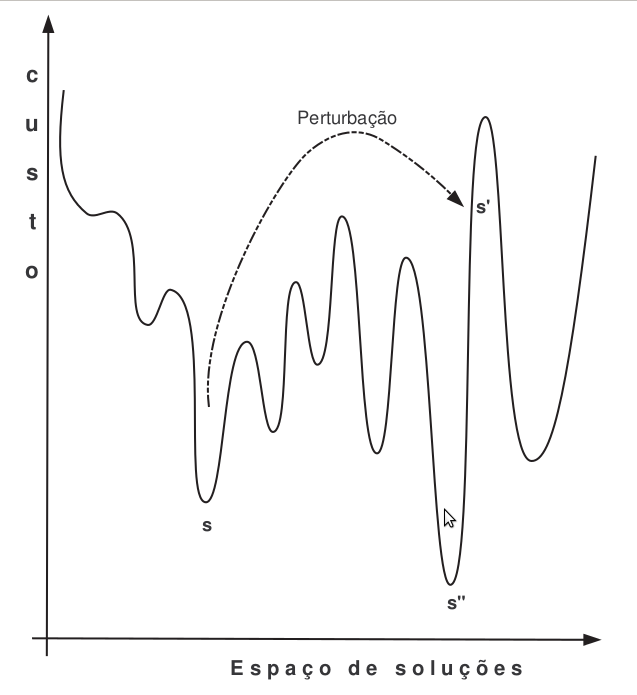
\includegraphics[scale=0.3]{./img/ilsfuncionamento.png}
	\caption{Representação esquemática do funcionamento do ILS}
	\label{img:ilsfuncionamento}
\end{figure}

A Figura \ref{img:ilsfuncionamento} demonstra o funcionamento do método ILS em um problema de minimização. Dado um ótimo local $s$, é realizada uma pertubação que lhe direciona para $s{'}$. Depois da aplicação da busca local, o novo mínimo $s{''}$, melhor que a anterior, é encontrada. Ou seja $f(s{''}) < f(s)$.

Uma exemplo de pertubação seria a aplicação sucessiva de estruturas de vizinhança a solução corrente.

\section{Programação Linear}

A programação linear é provavelmente a mais conhecida e utilizada técnica de otimização em todo o mundo. É geralmente utilizada para tomada de decisões gerenciais sobre a alocação de recursos para produção. Os custos dos recursos e as receitas geradas pelos produtos são usados para determinar a melhor solução. Qualquer problema que possa ser formulado com variáveis de decisão reais, tendo uma função-objetivo linear, e funções de restrição lineares, em princípio pode ser solucionado através da programação linear. Tais programas originariamente utilizavam o método \textit{Simplex}, porém, mais recentemente, métodos de "\textit{pontos interiores}" se mostraram mais eficientes.

Embora a programação linear seja muito eficiente para a resolução de problemas lineares, sua aplicação a problemas que apresentem objetivos ou restrições não-lineares tem levado a problemas e falhas de modelagem. Em alguns casos, funções não-lineares podem ser aproximadas por algumas funções lineares conjugadas, e a programação linear ainda pode ser utilizada. Contudo, isso leva a uma representação ineficiente do problema, podendo causar matrizes de decisão explosivamente grandes que demandam um tempo excessivo para resolução. Esta é uma dificuldade comum em problemas que envolvem, por exemplo, "\textit{scheduling}" e "\textit{sequenciamento}" de processos.

De forma equivalente, outros tipos de variáveis não podem ser tratadas diretamente com o uso de programação linear. Programação inteira usa programação linear para resolver problemas sobre variáveis inteiras, mas ainda com funções objetivo e restrições puramente lineares. As variáveis inteiras são representadas como variáveis reais no algoritmo de resolução do problema. Então um processo repetitivo é usado para "delimitar" o valor destas variáveis em valores inteiros, através da adição de restrições e reprocessamento da solução. Esse método, conhecido como \textit{"branch \& bound"}, finaliza quando todas as variáveis assumem valores inteiros. Quando o número de variáveis inteiras é pequeno, a programação inteira soluciona o problema rapidamente. Infelizmente esse procedimento pode consumir muito tempo com um número grande de variáveis inteiras, podendo, em alguns casos, necessitar de milhões de iterações para serem resolvidos.
 	
 	Essa técnica foi muito utilizada na segunda guerra mundial para otimizar as perdas inimigas e reduzir o custo das operações e também é utilizado no planejamento de algumas empresas.

\section{Revisão da literatura}
	
		O Trabalho de Argüello e Bard \citep{arguelo1007} (1997) resolve a parte de reconstrução de uma solução do PCTA que tenha sido corrompida por causa de atrasos e impedimentos de voos que ocorrem durante a execução de uma malha. Ele resolve esse problema utilizando a metaheurística GRASP, gerando vizinhos da solução atual de forma sucessiva até obter uma que seja considerada suficientemente boa.
		
		Mercier e Soumis \cite{mercier2007} (2007) resolveram o PCTA em conjunto com o problema de escala de tripulantes pois Cordeau et al. \cite{cordeau2001}, Klabjan et al. \cite{klabjan2002} e Cohn e Barnhart \cite{mainville2003} mostraram que a resolução desses problema de forma integrada pode gerar soluções que são significantemente melhor que as geradas de forma sequencial. O Modelo matemático proposto em CITAR AQUI foi adaptado para auxiliar na geração da nossa solução. 
		
		Em \cite{mohamed2011} Mohamed et al. resolveu de forma integrada o problema de atribuição de frota e o problema de construção de trilhos de aeronaves, para uma pequena empresa de aviação a TunisAir. Além disso as restrições de manutenção não foram levadas em consideração pelo fato dela poder ser feita em todos os aeroportos em que as aeronaves passam a noite.
		
%GRASPs have been used to find high quality solutions to a variety of logistics and combi- natorial optimization problems including maintenance base %planning (Feo and Bard, 1989), machine scheduling (Feo et al., 1991), and number partitioning (Argu ̈ello et al., 1996) to name a few.

\chapter{Geração das instâncias}
  
  Atualmente existem diversas fontes na qual se podem obter instâncias para problemas de otimização combinatória sendo uma das mais conhecidas a OR-Library \footnote{ pode ser acessado em http://people.brunel.ac.uk/~mastjjb/jeb/info.html} que foi descrito inicialmente descrito em J.E.Beasley \cite{orlibrary} permitindo o acesso a centenas de conjuntos de instâncias a partir da Internet. 
  
Apesar da existência dessas entidades não foi encontrado nenhuma instância que fosse compatível com o problema de construção de trilhos de aeronaves, fazendo-se então necessário a criação de um conjunto de instâncias próprias que além de permitir a conclusão desse presente trabalho ainda servirá como base para futuras propostas.
  
A obtenção de dados foi feita através da seleção manual do conjunto de voos domésticos cobertos pela empresa de transporte aéreo brasileira denominada TAM (http://www.tam.com.br/) que tinham o tempo de partida na segunda feira e se utilizava do equipamento AirBus Industrie A319. A segunda-feira foi identificada como sendo o dia 0 (zero) apenas para permitir sua utilização no algoritmo. Essa instância que foi obtida é composta por X voos e possui uma grande quantidade de ligações entre os Y aeroportos envolvidos tornando o grau de complexidade mais elevado que instâncias com a características hub-and-spoke que é mais comum nas malhas comerciais norte-americanas. Uma malha é considerada como sendo hub-and-spoke quando existe uma grande concentração de vôos em poucos aeroportos como pode ser visto na Figura K.
  
Para se obter um limite inferior dessas instâncias foi feita uma verificação com o algoritmo do Anexo X que permite checar a quantidade mínima de vôos que colidem em uma determinada janela de tempo que é definida pelo atraso máximo permitido. (Pode-se fazer uma formula para explicar esse funcionamento). Essa quantidade é dito como sendo o limite inferior da instância e é garantido que não existe solução com uma melhor quantidade de trilhos que essa sem que nenhum vôo seja excluído.
  
	A TAM tinha disponível nessa época com N aeronaves desse tipo, logo acreditamos que esse é o número de aeronaves que era necessário para atender a todos esses vôos, fazendo com que reduzir essa quantidade de vôos se tornasse um dos objetivos desse trabalho.
  
	Diversas instâncias também foram geradas a partir dessa, variando o número de voos e as características das malhas  com a finalidade de gerar instâncias com um variado grau de complexidade. Essas instâncias podem ser vistas no Anexo N e podem ser solicitadas diretamente com o autor, porém existe a intenção de adicionar esse conjunto de instâncias na OR-Library.
  
	Ainda é necessário a adição de outras instâncias reais para que a validação dos resultados se tornem mais práticos, para isso é necessário a colaboração de empresas de transporte aéreo uma vez que a obtenção desses dados por meios manuais se mostrou demorado e trabalhoso. 
  
  \chapter{Modelo matemático}\label{cap:modelomat}
  
A idéia utilizada nesssa formulação é que não há necessidade de
modelar os 4 tipos de arcos para cada voo. Para dois voos quaisquer existem
apenas 2 tipos de arcos que podem vir ocorrer como ilustrado na Figura
\ref{fig:modelagem_arcos}.

Em a) os voos respeitam a restrição geográfica, dessa forma apenas os arcos de
tipo 1 e 2 precisam ser modelados uma vez que não teria sentido fazer um voo de
reposicionamento nessa situação. Em b) os aeroportos em questão são diferentes,
sendo necessário apenas a modelagem dos arcos do tipo 3 e 4, perceba que não
teria outra saída se não efetuar um voo de reposicionamento.

\begin{figure}[ht]
	\centering
	\caption{Arcos necessários para ligar dois voos. \mbox{Fonte:
	(Própria)}}\label{fig:modelagem_arcos}
	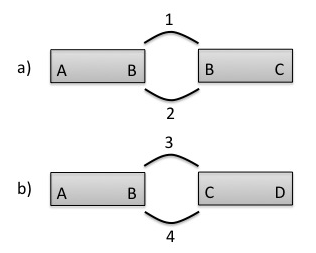
\includegraphics[scale=0.4]{./img/modelagem_arcos}
\end{figure}

Seja $D = (V,A)$ um grafo representando uma instância do PCTA, onde o conjunto de vértice $V = {v_{i}:i \in I}$ de D é indexado por $I = {1, 2, ..., n+1, n+2}$ onde $v_{n+1}$ e $v_{n+2}$, identificam, respectivamente, os nós fonte e destino. E os nós restantes referem-se ao conjunto de arcos originais, com $n$ elementos. Seja os custos ${c_{ij}:(i,j) \in A}$ introduzidos acima, estando associados com cada arco da instância.
  
Seja ${x_{ij}:(i,j) \in A}$ um conjunto binário 0-1 de variáveis usada para controlar a inclusão $(x_{ij} = 1)$ ou a exclusão $(x_{ij} = 0)$ de um arco (possível conexão) entre vértices (voos) $v_{i}$ e $v_{j}$. O conjunto $\overline{I}$ identifica o conjunto de nós excluindo o nó fonte $(v_{n+1})$ e o nó de destino $(v_{n+2})$. Variáveis reais $\delta_{i}$ e $\theta_{i}$, $i \in \overline{I}$ são usados para representar, respectivamente, o desvio do tempo de partida sugerido e a norma desse desvio para $v_{i}$. Essas variáveis devem no entanto obedecer $-\gamma_{i} \geq \delta_{i} \geq \gamma_{i}$ e $0 \geq \theta_{i} \geq \gamma_{i}$, onde $\gamma_{i}$ é o valor máximo de desvio permitido (em cada direção) do tempo de partida sugerido para o voo. Finalmente o tempo de partida sugerido que é dado por $s_{i}:i \in \overline{I}$.
  
\section{Função objetivo}

\begin{equation}
Minimizar \   \ \sum_{i \in I} \sum_{j \in I} x_{ij}c_{ij} + \sum_{i \in \overline{I}} \theta_{i}
\end{equation}

\section{Restrições}

\begin{enumerate}


\item[a)] Garantia de recobrimento dos voos \\
\begin{equation}
  \sum_{i \in I} x_{ij}= 1 \   \ \forall_{j} \in \overline{I} 
\end{equation}
\begin{equation}
\sum_{j \in I} x_{ij} = 1 \   \ \forall_{i} \in \overline{I}
\end{equation}





\item[b)] Viabilidade das conexões \\
\begin{equation}
s_{i} + t_{i}x_{ij} - INF(1 - x_{ij}) + \delta_{i} \leq s_{j} + \delta_{j} \   \ \forall_{i,j} \in \overline{I}
\end{equation}
%\begin{equation}
%\sum_{i \in I} x_{i(n+1)} = 0
%\end{equation}
%\begin{equation}
%\sum_{j \in I} x_{(n+2)j} = 0
%\end{equation}

\item[c)] Modulo do desvio do tempo de partida sugerido \\
\begin{equation}
\theta_{i} \geq \delta_{i} \   \ \forall_{i} \in \overline{I}
\end{equation}
\begin{equation}
\theta_{i} \geq -\delta_{i} \   \ \forall_{i} \in \overline{I}
\end{equation}

\item[d)] Limites das variáveis \\
\begin{equation}
-\gamma_{i} \geq \delta_{i} \geq \gamma_{i} \   \ \forall_{i} \in \overline{I}
\end{equation}
\begin{equation}
0 \geq \theta_{i} \geq \gamma_{i} \   \ \forall{i} \in \overline{I}
\end{equation}
\end{enumerate}

\clearpage

Pode-se perceber que o modelo matemático não faz menção ao tempo de solo ($g$), isso ocorre porque esse tempo é incorporado ao voo como demonstrado na Figura \ref{fig:conversion}, ou seja o tempo de partida sugerido $s$ passa a ter o valor $s - g$ e a duração $t$ do voo passa a ter o valor $t + g$. Uma vantagem de usar essa abordagem que integra o tempo de solo ao voo é que a quantidade de restrições é reduzida.

\begin{figure}[ht]
	\centering
	\caption{Conversão de um voo para ser utilizado no
	solver. \mbox{Fonte: (Própria)}}\label{fig:conversion}
	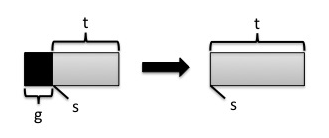
\includegraphics[scale=0.4]{./img/conversion}
	
\end{figure}

Além disso o conjunto $A$ contém apenas um tipo de arco, o arco do tipo 1 se os voos satisfazem a restrição geográfica e o arco do tipo 3 caso não satisfaçam. Os arcos do tipo 2 e 4 são modelados a partir  da variável $\delta$ que tem seu custo acrescentado na função objetivo.

Essa estratégia permite a redução de 3 arcos para cada voo, o que deixa o modelo mais leve.

O calculo dos custos são feitos através de um pré-processamento, onde os arcos viáveis recebem os valores referentes ao seu tipo, por exemplo, no caso de um arco originário do nó source, arco do tipo 6, um custo 1000 é atribuído. No caso de arcos que deverão ser evitados um custo elevado é atribuído.
  	
\chapter{Método Proposto} \label{cap:metodoprop}
  
O método proposto se utiliza do GRASP, do ILS e da abordagem exata através da
programação linear inteira, pretendendo tirar proveito das vantagens de cada
uma dessas técnicas. Ou seja, combinando a agilidade dos métodos heurísticos com
a optimalidade do método exato.
  
Da mesma forma que em outras abordagens heurísticas, esse novo algoritmo
consome pouco tempo computacional, em relação ao método exato e tem a capacidade
de escapar de mínimos locais.
  
O GRASP foi utilizado como a base do algoritmo, onde a parte da construção
seguiu a sua definição padrão, com a geração de uma lista restrita de candidatos
(LRC) e a posterior escolha aleatória entre esses elementos. A parte da busca
local foi adaptada para executar em conjunto com o ILS modificado. Para o ILS
foram definidos algumas estruturas de vizinhança que foram utilizadas
na busca local, e a perturbação foi feita com a utilização de um \textit{solver}
em uma parte do problema. Essa abordagem permite que o algoritmo gere boas
soluções e escape de mínimos locais além de promover uma aceleração na obtenção
de boas soluções, pois quando o \textit{solver} encontra uma melhor solução ele
consegue mudar o espaço de soluções em que a busca era efetuada.


O \textit{solver} é utilizado para resolver um modelo matemático que foi
desenvolvido baseado na proposta de \cite{pontes2002} que é aplicado a uma parte do problema cada
vez que se deseja fazer uma perturbação. Enquanto a busca local usa o método de
descida, variando entre três estruturas de vizinhança, o \textit{swap-x}, o
\textit{crossover} e a \textit{compactação}. Mais adiante serão dado mais
detalhes sobre o modelo matemático, a forma de escolha do sub problema, da fase
de construção que foi implementada, da busca local e das implementações que não
tiveram êxito.

\section{Modelo matemático} \label{sec:modelomat}

   
A modelagem proposta por \cite{pontes2002} aborda todas as restrições do
problema fazendo com que a quantidade de restrições geradas seja muito elevada.
A idéia utilizada na nossa formulação é a de tentar reduzir ao máximo a
quantidade de restrições necessárias. Isso é feito com a modelagem de apenas
algumas restrições, aquelas que são possíveis no mundo real.

Primeiro se percebeu que não há necessidade de modelar os 4 tipos de arcos para
cada voo, uma vez que dados dois voos só pode vir a ocorrer dois tipos de arcos
possíveis entre eles. Essa situação é ilustrada na Figura
\ref{fig:modelagem_arcos}.

\begin{figure}[ht]
	\centering
	\caption{Arcos necessários para ligar dois voos. \newline \mbox{Fonte:
	(Própria)}}\label{fig:modelagem_arcos}
	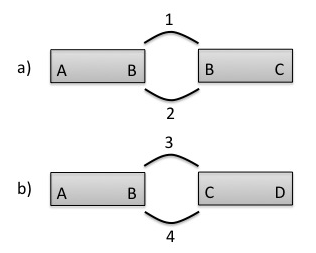
\includegraphics[scale=0.4]{./img/modelagem_arcos}
\end{figure}


Em a) os voos respeitam a restrição geográfica, dessa forma apenas os arcos de
tipo 1 e 2 precisam ser modelados uma vez que não teria sentido fazer um voo de
reposicionamento nessa situação. Em b) os aeroportos em questão são diferentes,
sendo necessário apenas a modelagem dos arcos do tipo 3 e 4, perceba que não
teria outra alternativa se não fazer um voo de reposicionamento.

\subsection{Definição}

Seja $D = (V,A)$ um grafo representando uma instância do PCTA, onde o conjunto
de vértice $V = {v_{i}:i \in I}$ de D é indexado por $I = {1, 2, ..., n+1,
n+2}$ onde $v_{n+1}$ e $v_{n+2}$, identificam, respectivamente, os nós fonte e
destino. E os nós restantes referem-se ao conjunto de nós originais, com $n$
elementos. Sejam os custos ${c_{ij}:(i,j) \in A}$ introduzidos acima, estando
associados com cada arco do grafo.
  
Seja ${x_{ij}:(i,j) \in A}$ um conjunto binário 0-1 de variáveis usada para
controlar a inclusão $(x_{ij} = 1)$ ou a exclusão $(x_{ij} = 0)$ de um arco
(possível conexão) entre vértices (voos) $v_{i}$ e $v_{j}$. O conjunto
$\overline{I}$ identifica o conjunto de nós excluindo o nó fonte $(v_{n+1})$ e
o nó de destino $(v_{n+2})$. A função objetivo foi dividida para facilitar o
entendimento de como é feito o custo de adicionar um trilho. Variáveis reais
$\delta_{i}$ e $\theta_{i}$, $i \in \overline{I}$ são usados para representar,
respectivamente, o desvio do tempo de partida sugerido e a norma desse desvio
para $v_{i}$. Essas variáveis devem no entanto obedecer $-\gamma_{i} \geq
\delta_{i} \geq \gamma_{i}$ e $0 \geq \theta_{i} \geq \gamma_{i}$, onde
$\gamma_{i}$ é o valor máximo de desvio permitido (em cada direção) do tempo de
partida sugerido para o voo. Finalmente o tempo de partida sugerido que é dado
por $s_{i}:i \in \overline{I}$.
  
\section{Função objetivo}

\begin{equation}
Minimizar \  \ \sum_{j \in \overline{I}} x_{v_{n+1}j}(CUSTO\_TRILHO) + \sum_{i \in
\overline{I}} \sum_{j \in I} x_{ij}c_{ij} + \sum_{i \in
\overline{I}} \theta_{i}
\end{equation}

\section{Restrições}

\begin{enumerate}


\item[a)] Garantia de recobrimento dos voos \\
\begin{equation}
  \sum_{i \in I} x_{ij}= 1 \   \ \forall_{j} \in \overline{I} 
\end{equation}
\begin{equation}
\sum_{j \in I} x_{ij} = 1 \   \ \forall_{i} \in \overline{I}
\end{equation}





\item[b)] Viabilidade das conexões \\
\begin{equation}
s_{i} + t_{i}x_{ij} - M(1 - x_{ij}) + \delta_{i} \leq s_{j} + \delta_{j} \   \ \forall_{i,j} \in \overline{I}
\end{equation}
%\begin{equation}
%\sum_{i \in I} x_{i(n+1)} = 0
%\end{equation}
%\begin{equation}
%\sum_{j \in I} x_{(n+2)j} = 0
%\end{equation}

\item[c)] Modulo do desvio do tempo de partida sugerido \\
\begin{equation}
\theta_{i} \geq \delta_{i} \   \ \forall_{i} \in \overline{I}
\end{equation}
\begin{equation}
\theta_{i} \geq -\delta_{i} \   \ \forall_{i} \in \overline{I}
\end{equation}

\item[d)] Limites das variáveis \\
\begin{equation}
-\gamma_{i} \geq \delta_{i} \geq \gamma_{i} \   \ \forall_{i} \in \overline{I}
\end{equation}
\begin{equation}
0 \geq \theta_{i} \geq \gamma_{i} \   \ \forall{i} \in \overline{I}
\end{equation}
\begin{equation}
x_{ij} \in \{0,1\}
\end{equation}
\end{enumerate}

\clearpage

Pode-se perceber que o modelo matemático não faz menção ao tempo de solo ($g$).
Isso ocorre pois esse tempo é incorporado ao voo como demonstrado na Figura
\ref{fig:conversion}, ou seja o tempo de partida sugerido $s$ passa a ter o
valor $s - g$ e a duração $t$ do voo passa a ter o valor $t + g$. Uma vantagem
de usar essa abordagem que integra o tempo de solo ao voo é a redução da
quantidade de restrições do problema.

\begin{figure}[ht]
	\caption{Conversão de um voo para ser utilizado no
	solver. \newline \mbox{Fonte: (Própria)}}\label{fig:conversion}
	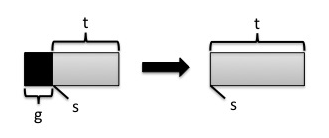
\includegraphics[scale=0.4]{./img/conversion}
	
\end{figure}

Além disso o conjunto $A$ contém apenas um tipo de arco, o arco do tipo 1 se os
voos satisfazem a restrição geográfica e o arco do tipo 3 caso não satisfaçam.
Os arcos dos tipos 2 e 4 são modelados a partir  da variável $\delta$ que tem
seu custo acrescentado na função objetivo.

Essa estratégia permite a redução de 3 arcos para cada voo, o que deixa o
modelo mais leve.

O calculo dos custos são feitos através de um pré-processamento, onde os arcos
viáveis recebem os valores referentes ao seu tipo, por exemplo, no caso de um
arco originário do nó origem, arco do tipo 6, um custo 1000 é atribuído. No
caso de arcos que deverão ser evitados um custo elevado é atribuído.
  	
  	
%\section{Pré-processmanto da instância}

%No caso da instância possuir mais de um dia de operação então pode-se quebra-la
%em dias se houver tempo vago entre os dias dessa instância.
  
\section{Fase de construção do GRASP}
  
A construção da solução é feita elemento a elemento utilizando o
GRASP. Inicialmente é feita a ordenação do conjunto de voos a partir do seu
tempo de partida sugerido. O algoritmo só termina quando todos os voos já
foram alocados em algum trilho.
  
Existem duas formas de fazer a montagem da solução, uma seria a montagem de
trilhos de forma sequencial, onde um novo trilho só é iniciado quando o anterior
se encontra saturado. A outra forma é a montagem de trilhos de forma paralela,
que, a priori, provocaria uma melhor distribuição dos voos. Na prática a
primeira abordagem foi adotada, pois, nas instâncias disponíveis ela apresentou,
sempre, soluções de melhor qualidade. 

Pode ser que para instâncias com alguma característica específica a
estratégia de montagem dos trilhos de forma paralela pode apresentar melhores
resultados.

\begin{figure}[h]
\caption{Pseudocódigo do procedimento de seleção de um voo inicial. \newline
\mbox{Fonte: Própria}}\label{alg:selectinit}
\begin{programma}
\ALGORITHM{selecionaVooInicial(V)}

\STATE $LCI$ \GETS cincoPrimeirosVoos($V$);
\STATE $h(v_{min}) \GETS min\{h(v) \mid v \in LCI\}$;
\STATE $h(v_{max}) \GETS max\{h(v) \mid v \in LCI\}$;
\STATE $LRI \GETS \{v \in LCI \mid h(v) \leq h(v_{min}) + \alpha(h(v_{max}) -
h(v_{min}))\}$;
\STATE Selecione aleatoriamente um elemento $v \in LRI$;
\STATE\RETURN $v$;
\ENDALGORITHM
\end{programma}
\end{figure}
  
\subsection{Formação dos trilhos de forma sequencial}

Quando se pensa na escolha do primeiro voo do trilho, a decisão imediata é a
escolha do voo que contenha o menor horário de partida sugerido, ou seja, o voo
mais próximo. Porém essa escolha reduz a quantidade de soluções que podem ser
geradas, isso ocorre pois o primeiro voo tem uma grande influência nas
possíveis soluções que um trilho pode assumir. Para evitar isso a escolha do
primeiro voo de um trilho é feita baseando-se nos 5 voos com menor horário de
partida que ainda não estejam alocados a nenhum outro trilho. 

Esses voos são adicionados a lista de candidatos iniciais (LCI) em seguida é
feita a escolha do elemento que irá iniciar o novo trilho levando em
consideração apenas os elementos que possuam o horário de partida distante de
até $\alpha \%$ do voo de menor horário de partida. Isso é feito para
evitar a escolha de um voo muito distante do menor voo.

\begin{figure}[h]
\caption{Pseudocódigo do procedimento de formação sequencial dos trilhos.
\newline
\mbox{Fonte: Própria}}\label{alg:formseq}
\begin{programma}
\ALGORITHM{construçãoSequencial(V)}

\STATE Ordene o conjunto de voos não alocados $V$;
\STATE $M \GETS \emptyset$;
\WHILE{$V \neq \emptyset$}
\STATE $v \GETS selecionaVooInicial(V)$
\STATE $T \GETS \{v\}$;
\STATE $T \GETS completaTrilho(T)$;
\STATE $V \GETS V - \{v \in T\}$;
\STATE $M \GETS M \cup T$;
\ENDWHILE
\STATE\RETURN $M$;

\ENDALGORITHM
\end{programma}
\end{figure}

\subsection{Formação dos trilhos de forma paralela}
 
Nessa estratégia um trilho é iniciado sempre que existe um voo que não pode ser
inserido em nenhum dos trilhos que estejam sendo montados, mantendo-se assim um
conjunto de trilhos disponíveis (CTD).

Em cada iteração o trilho corrente (TC) é escolhido a partir do CTD de forma
aleatória. Feito isso, adiciona-se um voo a esse trilho. Caso não existam voos
candidatos para adição no TC este é removido da CTD e uma nova iteração é
iniciada.

\begin{figure}[h]
\caption{Pseudocódigo do procedimento de formação paralela dos trilhos.
\newline
\mbox{Fonte: Própria}}\label{alg:formparalel}
\begin{programma}
\ALGORITHM{construçãoParalela(V)}

\STATE Ordene o conjunto de voos não alocados $V$;
\STATE $M \GETS \emptyset$;
\STATE $CTD \GETS \emptyset$;
\WHILE{$V \neq \emptyset$}
\STATE $v \GETS selecionaVooInicial(V)$
\IF {$v$ pode ser inserido em um trilho do CTD}
	\STATE $TC \GETS escolheTrilhoAleatório(CTD)$;
	\STATE $nv \GETS selecionaVooCandidato(TC)$;
	\IF {$nv = \emptyset$}
		\STATE $CDT \GETS CDT - \{TC\}$
		\STATE $M \GETS M \cup \{TC\}$
	\ELSE
		\STATE $TC \GETS TC \cup \{nv\}$
	\ENDIF
\ELSE
	\STATE $T \GETS \{v\}$; 
	\STATE $CTD \GETS CTD \cup T$ 	
\ENDIF
\ENDWHILE

\STATE $M = M \cup \{t \in CTD\}$;
\STATE\RETURN $M$;

\ENDALGORITHM
\end{programma}
\end{figure}

\begin{figure}[h]
\caption{Pseudocódigo de calculo do proximo voo de um trilho
\newline
\mbox{Fonte: Própria}}\label{alg:calcvoo}
\begin{programma}
\ALGORITHM{obtemProximoVoo(T,V)}

\STATE $A \GETS \{1,2,3,4\}$;
\STATE $a \GETS sorteaTipoDeArco(TiposDeArco, P_{1},P_{2},P_{3},P_{4})$;
\STATE $A \GETS A - \{a\}$;
\STATE $v \GETS ultimoVoo(T)$;

\FOR{$i$ \FROM $1$ \TO $4$}\PGlnlabel{forline}
\STATE $c \GETS proximoCandidato(v, V, a)$;
\IF {$c = \emptyset$}
	\STATE $a \GETS proximoArco(A)$;
	\STATE $A \GETS A - \{a\}$;
\ELSE
	\STATE\RETURN $c$;
\ENDIF 
\ENDFOR

\STATE\RETURN $\emptyset$;

\ENDALGORITHM
\end{programma}
\end{figure}
  
\subsection{Escolha dos voos de um trilho}

A escolha do primeiro voo de um trilho é feita como explicado nas seções
anteriores enquanto os demais voos são escolhidos tendo como base um tipo de
arco e uma lista restrita de candidatos (CLR).
 
Os tipos de arcos foram definidos no Capítulo \ref{cap:descprob}, porém nessa
etapa apenas 4 tipos são considerados, o   $A_{1},A_{2},A_{3},A_{4}$ que
representam formas de ligações entre os voos. Os arcos do tipo 5 e 6 só são
utilizados na modelagem matemática. Os arcos do tipo 1 permitem a
ligação de voos sem a utilização de atrasos e/ou reposicionamentos. Os arcos do
tipo 2 utilizam atrasos mas não o reposicionamento. Os arcos do tipo 3 permitem
o sequenciamento com a utilização de um voo de reposicionamento mas sem inserir
atraso em nenhum dos voos envolvidos. Os arcos do tipo 4 utilizam-se de atrasos
e de um voo de reposicionamento para fazer a ligação entre dois voos. Os arcos
do tipo 5 pargem do nó \textit{source} e servem para modelar o inicio de um
trilho. Os arcos do tipo 6 tem chegam ao nó \textit{sink} e indicam o fim de um
trilho.

Primeiramente é feita a escolha do tipo de arco que será utilizado para efetuar
a ligação do ultimo voo do trilho corrente. Essa escolha é feita tendo
como base as probabilidades de cada um desses arcos acontecer. Essa
probabilidade foi definida como sendo
$P(A_{1})=0.79,P(A_{2})=0.16,P(A_{3})=0.04,P(A_{4})=0.01$ pois a solução ótima
do problema real da Rio Sul apresentava essas características. Esses valores
são empíricos e para determinadas instâncias podem gerar melhores soluções se
alterados.

De posse do tipo de arco, é feita então a formação da lista de candidatos. Essa
lista é ordenada de acordo com o seu horário de partida sugerido, caso o arco
seja do tipo $A_{1}$, ou pelo custo associado a sua escolha para os demais
tipos de arco. No caso da lista de candidatos não possuir nenhum voo, então
outro tipo de arco é sorteado, até que não seja possível acrescentar voos ao
trilho de nenhuma forma, quando isso ocorrer a construção
desse trilho é finalizada.
 
Caso seja possível a obtenção de uma lista de candidatos então ela é reduzida
tendo como base o passo 4 a 6 do algoritmo \ref{alg:graspcons} formando assim a
lista de candidatos restrita (LCR), essa redução remove os candidatos que estão
muito afastado do melhor candidato da lista. Como está lista se encontra
ordenada, então, o elemento de menor impacto ($v_{menor}$) na solução é o
primeiro e o de maior impacto ($v_{maior}$) é o último. A LCR contém os
candidatos que tenha o valor de impacto na solução de até $valor_{menor} +
\alpha*(valor_{maior} + valor_{menor})$, onde $\alpha$ é o grau de
gulosidade do GRASP. O candidato deve ser escolhido de forma aleatória entre os
elementos da LCR.
 
 \section{Fase de busca local do GRASP}

Com a finalização da etapa anterior tem-se uma solução do problema. A fase de busca
local efetua modificações nessa solução com a finalidade de obter outras
melhores que estejam próximos a ela, isso é feito através da aplicação das
estruturas de vizinhanças. No método proposto essa fase foi implementada através
da utilização da metaheurística ILS que alterna busca local com pertubações
conseguindo assim escapar de mínimos locais quando não consegue mais melhorar a
solução, ou seja, primeiro são aplicados as estruturas de vizinhança, visando
obter o valor ótimo local da solução, depois é feita uma perturbação que
diversifica melhorando o valor da função objetivo através da aplicação do
modelo matemático que foi desenvolvido em uma parte do problema. Quando nenhuma
das duas estratégias consegue melhorar a solução então a busca local encerra e
uma nova iteração do GRASP pode ser iniciada.
 
\subsection{Estruturas de vizinhança}
 
Foram definidas três estruturas de vizinhança para serem utilizadas na busca
local, o Swap-X e o Cross-Over, que tem o objetivo de remover modificações nos
horários de partida sugeridos dos voos, e a Compactação, que promove a redução
do número de trilhos. Abaixo essa estruturas são explicadas.
 
\subsubsection{Swap-X}

Esse operador efetua a troca de X voos de um trilho por um conjunto de voos de
outro trilho. Dessa forma pode-se conseguir remover os atrasos que foram criados
na etapa de construção. No método proposto apenas os movimentos do tipo Swap-1
e Swap-2 são utilizados, pois essa vizinhança é considerada grande. Na Figura
\ref{fig:swap1} um caso de melhoria no custo dos trilhos é exemplificada.

\begin{figure}[ht]
	\caption{Estrutura de vizinhança Swap-1. \newline \mbox{Fonte:
	(Própria)}}\label{fig:swap1}
	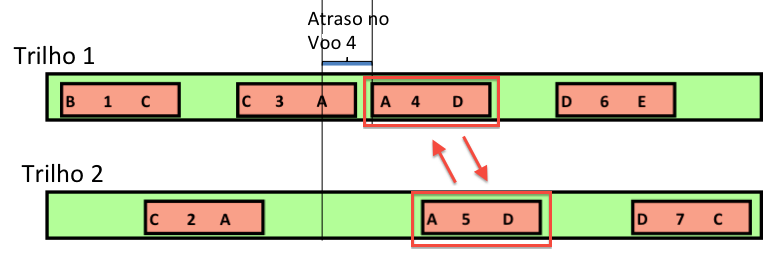
\includegraphics[scale=0.4]{./img/swap-1}
	
\end{figure}
 
 \subsubsection{Cross-Over}
 
A ideia do operador $crossover$ é a de efetuar troca entre dois segmentos de
trilhos com a finalidade de gerar novos trilhos com menos modificações no
horário de partida. A Figura \ref{fig:crossover} ilustra uma melhoria causada por um
movimento desse tipo.


\begin{figure}[ht]
	\caption{Estrutura de vizinhança CrossOver. \newline \mbox{Fonte:
	(Própria)}}\label{fig:crossover}
	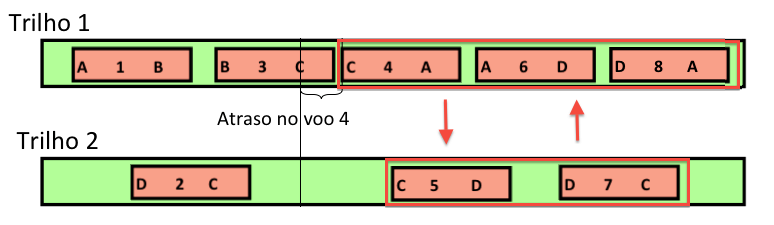
\includegraphics[scale=0.4]{./img/crossover}
	
\end{figure}
 
 \subsubsection{Compactação}
 
A compactação é a única estrutura de vizinhança utilizada que é capaz de
reduzir a quantidade de trilhos da solução final.
 
Isso ocorre porque ela consegue, insere um trilho em outro de forma direta ou
com a utilização de um voo de reposicionamento.
 
A figura \ref{fig:compactacao} mostra a redução de um trilho com a utilização
desse movimento.

\begin{figure}[ht] 
	\caption{Estrutura de vizinhança Compactação. \newline \mbox{Fonte:
	(Própria)}}\label{fig:compactacao}
	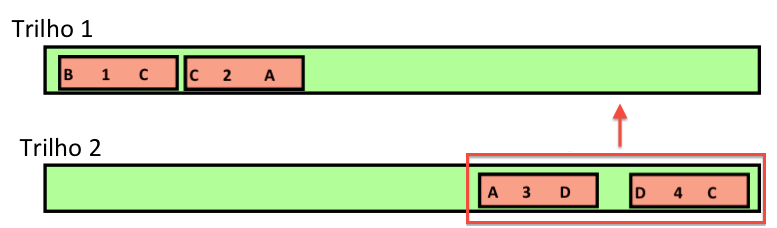
\includegraphics[scale=0.4]{./img/compactacao}
	
\end{figure}
 
 \subsection{Perturbação usando o método exato}
   
A perturbação normalmente é utilizada quando as estruturas de vizinhança não
conseguem melhorar a solução, quando isso ocorre, pode-se dizer que a
solução corrente é a ótima local com relação a vizinhança que foi definida.
 
Para tentar encontrar outros mínimos locais aplica-se uma modificação na
estrutura da solução, mesmo que isso provoque uma piora na sua qualidade. Isso
se mostra interessante para o algoritmo pois ele irá efetuar busca de melhorias
em outros locais no espaço de soluções através da sua busca local.
 
O método de perturbação utilizado aqui difere do que normalmente é aplicado
pois a solução tem a sua estrutura modificada e ainda consegue melhorar a sua
qualidade. Isso é feito através da aplicação do modelo matemático em uma
parte do problema. A sua utilização ocorre com a seleção de um conjunto de
trilhos, e sua a posterior aplicação no solver com o modelo desenvolvido
configurado para o conjunto de voos da seleção.

O método exato retorna a configuração ótima desses voos, que
são agrupados novamente a solução antiga. O solver tem um tempo máximo
estabelecido e se não retornar nenhuma solução considera-se que não houve
melhora sua aplicação.

A seleção dos trilhos é feita com base no seu
\textit{grau de compactação} que é definido como sendo porcentagem de
utilização efetiva de um trilho com relação ao tempo de partida do primeiro voo
e o tempo de chegada do último voo da instância, ou seja, quanto maior o tempo
que a aeronave, que opera um determinado trilho, permanece voando maior será o
seu grau de compactação. O calculo do grau de compactação não leva em
consideração os voos de reposicionamento, pois eles não estão no planejamento
inicial e por sua vez não são passados para o modelo.

Existe três formas de fazer a seleção dos trilhos que serão aplicados no solver,
pode-se adicionar os trilhos que possuem o maior grau de compactação, pode-se
adicionar os trilhos que possuem o menor grau de compactação ou pode-se alternar
entre a escolha de um trilho com o maior grau de compactação e um de menor grau
de compactação.

Na prática adotou-se a segunda abordagem, selecionando os trilhos de menor grau
de compactação, pois os resultados foram melhores.
 
Os trilhos são adicionados a solução até o limite de 80 voos, pois o solver
conseguiu em nossos experimentos resolver um problema desse porte de forma
imediata. 


 
   
  \chapter{Resultados preliminares e discursões}

Todos os algoritmos descritos foram desenvolvidas na linguagem C++ usando a biblioteca CPLEX Academic 12 para implementar o mecanismo de programação inteira. Todos os experimentos computacionais foram feitos em um notebook com a seguinte especificação: Pentium T4500 2.3 Ghz com 2 GB de RAM e rodando o sistema operacional sistema operacional Linux Ubuntu 11.04.

Foram efetuadas 10 iterações do GRASP usando um $\alpha$ de 0.5 e a busca local finalizava quando não conseguia melhorar o resultado. Para demonstrar a eficiência dos resultados foram realizadas comparações com o resultado ótimo obtido com um procedimento de programação inteira implementando o modelo descrito no capítulo \ref{cap:descprob}. A coluna $s*$ indica o valor ótimo. O método híbrido foi executado 20 vezes e apenas a média dos valores obtidos foram levados em consideração. A coluna $s$ indica a média dos valores obtidos com a execução do algoritmo, a coluna tempo indica a média da duração das execuções em segundos. A coluna final indicada por $GAP$ indica a diferença percentual das soluções e é calculado como segue:

\[  GAP = (s* - s)/s \]

Para os testes foram utilizados duas instâncias diárias, uma da Rio-Sul(107 voos) e outra da TAM (241 voos).  Com a finalidade de permitir estimar o tempo computacional necessário para resolver instâncias maiores foi proposto a extensão da frequência dos voos da instância Rio-Sul para uma semana, dessa forma foi gerado uma instância com 749 voos. Para simplificar foram adotados o tempo de solo de 20 minutos para todos os aeroportos.

A resolução dessas instâncias foram parametrizadas levando em consideração dois cenários. O cenário 1 faz o sequênciamento dos voos sem a permissão de utilizar nenhum atraso, essa representação é comum nas companhias que não aceitam a modificação do planejamento inicial. O cenário 2 se utiliza de atrasos permitindo assim uma maior liberdade na hora da montagem dos trilhos. Os parâmetros utilizados são detalhados na Tabela \ref{tab:params}.

\begin{table}
\caption{Parametrização dos cenários}\label{tab:params}
\begin{center}


\begin{tabular}{l|rr}
\hline

 & Cenário 1 & Cenário 2 \\
 \hline
 Atraso Maximo & 0 & 10 \\
 Prob. Arc. Tipo 1 & 0.92 & 0.69\\ 
 Prob. Arc. Tipo 2 & 0 & 0.16\\
 Prob. Arc. Tipo 3 & 0.08 & 0.04 \\
 Prob. Arc. Tipo 4 & 0 & 0.01 \\
  
\hline

\end{tabular}
\end{center}
\end{table}

 
%A Tabela \ref{tab:cenario1} e \ref{tab:cenario2} mostram os resultados as melhores soluções obtidas. No caso dos problemas diários e da instância da Rio Sul estendida a utilização do solver é suficiente e retorna o resultado ótimo em um tempo totalmente aceitável, dessa forma o método está sendo desenvolvido parar a resolução de problemas de grande porte. No caso de problemas reais isso iria refletir nas frotas mais comuns das companhias aéreas, que é onde se encontra a maior demanda de passageiros. Caso alguma informação extra seja necessária os anexos \ref{anx:netriosul} a \ref{anx:resulttam} apresentam a descrição completa das instâncias e das soluções que foram obtidas, 


%Rio Sul & 17.138 & 17 & 0 & 2 & XX & XX & 0\\
%TAM & 35.334 & 34 & 0 & 10 & XX & XX & 0 \\
%Rio Sul Estendida & 18392 & 17 & 0 & 20 & XX & XX & 0\\
%TAM Estendida & XX & XX & XX & XX & XX & XX & XX \\

\begin{table}[ht]
\caption{Resultados do cenário 1}\label{tab:cenario1}
\begin{center}


\begin{tabular}{l r r r r}
\hline

Instância & BKS & Resultado & Tempo(s) & GAP \\
\hline

Rio Sul & 17.138 & 17.138 & 4.8 & 0\\
TAM & 35.334 & 35.348 & 37 &  0.0004\\
Rio Sul Estendida & 18.392 & 21.911 & 525 & 0.19\\
%TAM Estendida & XX & XX & XX & XX \\

\hline
\end{tabular}

\end{center}
\end{table}

\begin{table}[ht]
\caption{Resultados do cenário 2}\label{tab:cenario2}
\begin{center}


\begin{tabular}{l r r r r}
\hline

Instância & BKS & Resultado & Tempo(s) & GAP \\
\hline

Rio Sul & 16.158 & 16.158 & 5 & 0\\
TAM & 35.015 & 35015 & 22 & 0 \\
Rio Sul Estendida & 17.433 & 20564 & 494 & 0.18\\ 
%TAM Estendida & XX & XX & XX & XX \\

\hline
\end{tabular}

\end{center}
\end{table}

	Pode-se observar que nos dois cenários a solução ótima foi obtida para a instância da Rio-Sul. Na instância da TAM a solução ótima foi encontrada, porém, na média o cenário 1 encontrou uma solução bem próxima. Essas duas instâncias representam um horizonte de tempo de um dia. Na instância da Rio-Sul estendida que representam uma semana de operação as soluções ficaram em média 0.19 do ótimo para o cenário 1 e 0.18 no cenário 2 com um tempo aproximado de 8 minutos. Para o procedimento programação linear não foram inseridos limites previamente calculados, de modo que a ferramenta utilizou apenas a relaxação linear.
  
 Alguns ajustes ainda podem melhorar o modelo híbrido para que ele possa se aproximar mais da solução ótima. A modificação da estrutura a ser otimizada na busca local pode ser um ponto que ajude a melhorar os resultados, pois a literatura mostra que esse é um dos pontos mais importantes de uma heurística híbrida.
 
 Uma das grandes dificuldades encontradas no trabalho foi a falta de instâncias na literatura tornando difícil a comparação de resultados com outras abordagens. Com isso existe a necessidade de geração de um conjunto de instâncias e a sua publicação para fins comparativos.
 
 Existe ainda a possibilidade de uma implementação paralela que ainda está em fase de planejamento e que se demonstrar resultados interessantes em tempo hábil será adicionada a dissertação.
 

%Com a eficiência obtida com o método exato existe uma necessidade de geração de instâncias maiores que possam ser utilizadas parar ajustar e justificar a utilização de uma abordagem mais complexa como o uso de uma metaheurística híbrida.

%Atualmente o método híbrido conseguiu resolver a instância \textit{TAM Estendida} com o tempo de 60s e Custo total de 43344, que parece %ser uma boa solução tendo como base os resultados obtidos com a instância que lhe serviu de base.

%Atualmente existe a necessidade de um melhor ajuste no método híbrido para que ele possa conseguir resultados mais robustos.

%A utilização de uma abordagem exata em conjunto com metaheurísticas está sendo cada vez mais utilizado na literatura. Porém a escolha da estrutura a ser otimizada deve ser bem escolhida para não aumentar demasiadamente a capacidade computacional necessária para resolver o problema.



%Para demonstrar a eficiência em termos de qualidade da solução da metaheurística GILS, realizamos comparações com um  procedimento exato B&B (XPRESS MP, 2004), implementando o modelo STSP apresentado por Lee (1996). Para cada instância da Tabela 1 temos as duas primeiras colunas representando as dimensões das instâncias testadas e as colunas restantes divididas em dois grupos: procedimento B&B e GILS. No caso do procedimento B&B, a coluna z* indica o valor ótimo e a coluna tempo indica o tempo computacional, em segundos, gasto na resolução da instância. Já para o grupo da metaheurística GILS as colunas adicionais, além da coluna tempo, são: iter que indica a iteração onde foi encontrada melhor solução, z que indica o valor obtido pelo GILS e, Δ (gap) que indica a diferença percentual entre as soluções:
%Δ = [ (z – z*) / z* ] x 100.


 % \chapter{Conclusões}
  
  %Os resultados obtidos, apesar de iniciais, indicam que existe um grande potencial na utilização desse conjunto de técnicas. O que ainda %é necessário é a construção ou a obtenção de uma maior quantidade de instâncias para permitir explorar e ajustar melhor diversos pontos do %método proposto.
  
 % A utilização de uma abordagem exata em conjunto com metaheurísticas está sendo cada vez mais utilizado na literatura. Porém a escolha da %estrutura a ser otimizada deve ser bem escolhida para não aumentar demasiadamente a capacidade computacional necessária para resolver o %problema.

\backmatter
  
\bibliographystyle{coppe-plain}
\bibliography{bibliografia}

\appendix
\chapter{Cronograma}

A seguir temos o cronograma das atividades que foram e que serão desenvolvidas no decorrer do curso de pós graduação.
    
\begin{figure}[ht]
	\centering
	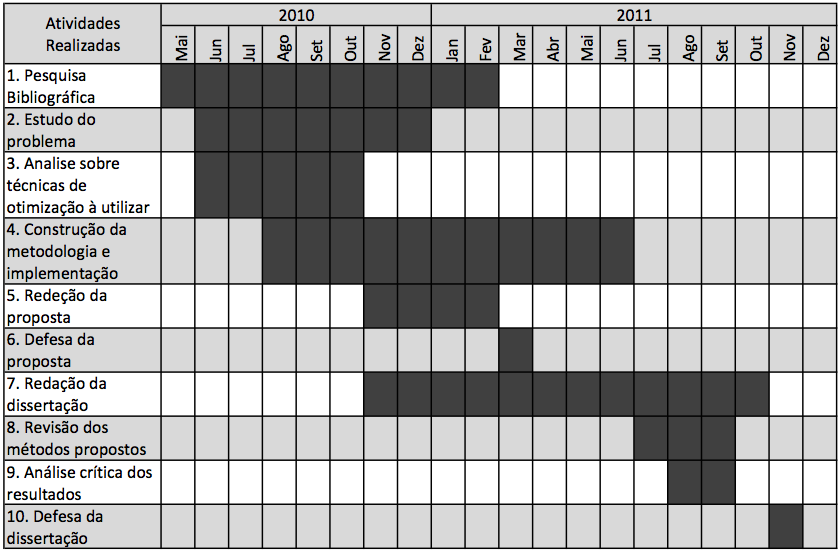
\includegraphics[scale=0.48]{./img/cronograma}
	%\caption{Heurística de construção aleatória de uma solução inicial}
	\label{cronograma}
 \end{figure}
    
Inicialmente foi feito um levantamento bibliográfico sobre o PCTA e outros que são correlatos ou similares a ele, também foi pesquisado sobre metaheurísticas que tiveram bons resultados com esses tipos de problemas. Em seguida foi estudado a possibilidade de integração da metaheurística escolhida com alguma modelagem matemática eficiente. Após isso foi elaborado e implementado o método proposto.

Fica faltando ainda a finalização dessa implementação e a revisão do método proposto, bem como a análise crítica dos resultados. Após isso segue-se a redação da dissertação para posterior defesa da mesma. O mês de dezembro de 2011 a fevereiro de 2012 ficam vagos para o caso de ocorrer algum imprevisto no decorrer da execução do cronograma.


\end{document}

